\documentclass[../notes.tex]{subfiles}

\pagestyle{main}
\renewcommand{\chaptermark}[1]{\markboth{\chaptername\ \thechapter\ (#1)}{}}
\setcounter{chapter}{7}

\begin{document}




\chapter{Crystal Structure and Surface Chemistry}
\section{X-Ray Diffraction Fundamentals}
\begin{itemize}
    \item \marginnote{5/16:}Final exam next Wednesday in class.
    \begin{itemize}
        \item 50 minutes.
        \item Questions like the midterm.
        \item We can bring our notes and textbook, but cannot search online.
        \begin{itemize}
            \item Can we bring notes on a computer, like mine, or do we have to print?
        \end{itemize}
        \item 1 computation problem.
        \item We will write answers on paper.
    \end{itemize}
    \item Review of last lecture.
    \item Tian goes through some examples of naming crystallographic planes from pictures of them intersecting a unit cell.
    \begin{itemize}
        \item The first example is a $111$ plane.
        \begin{itemize}
            \item If asked to identify a $111$ plane, it is enough to identify it as a $111$ plane; we do not have to identify it as a possible $222$ plane, too.
        \end{itemize}
        \item Consider a plane intersecting the \textbf{a}, \textbf{b}, and \textbf{c} axes at $a'=2a/5$, $b'=b/2$, and $c'=c/5$, respectively.
        \begin{itemize}
            \item Then $h=\frac{5}{2}$, $k=2$, and $l=5$.
            \item An easier way to show this, however, is with $h=5$, $k=4$, and $l=10$. Aren't these planes spaced twice as close together, though?
        \end{itemize}
        \item Consider a plane intersecting the \textbf{a}, \textbf{b}, and \textbf{c} axes at $a'=a/2$, $b'=b/2$, and $c'=-c/4$, respectively.
        \begin{itemize}
            \item A convenient point to use as the origin in this case is the upper-left corner.
            \item Thus, the plane is $(2,2,-4)$.
            \item The question of could we denote the plane by $(1,1,-2)$: These two sets of planes are parallel, but the spacing of $(1,1,-2)$ would skip every plane like $(2,2,-4)$. Thus, we need $(2,2,-4)$ for the spacing.
        \end{itemize}
    \end{itemize}
    \item Rules.
    \begin{enumerate}
        \item If you see a fraction, convert to integers.
        \item But do not reduce a ratio.
    \end{enumerate}
    \item The fundamentals of X-ray diffraction.
    \begin{figure}[H]
        \centering
        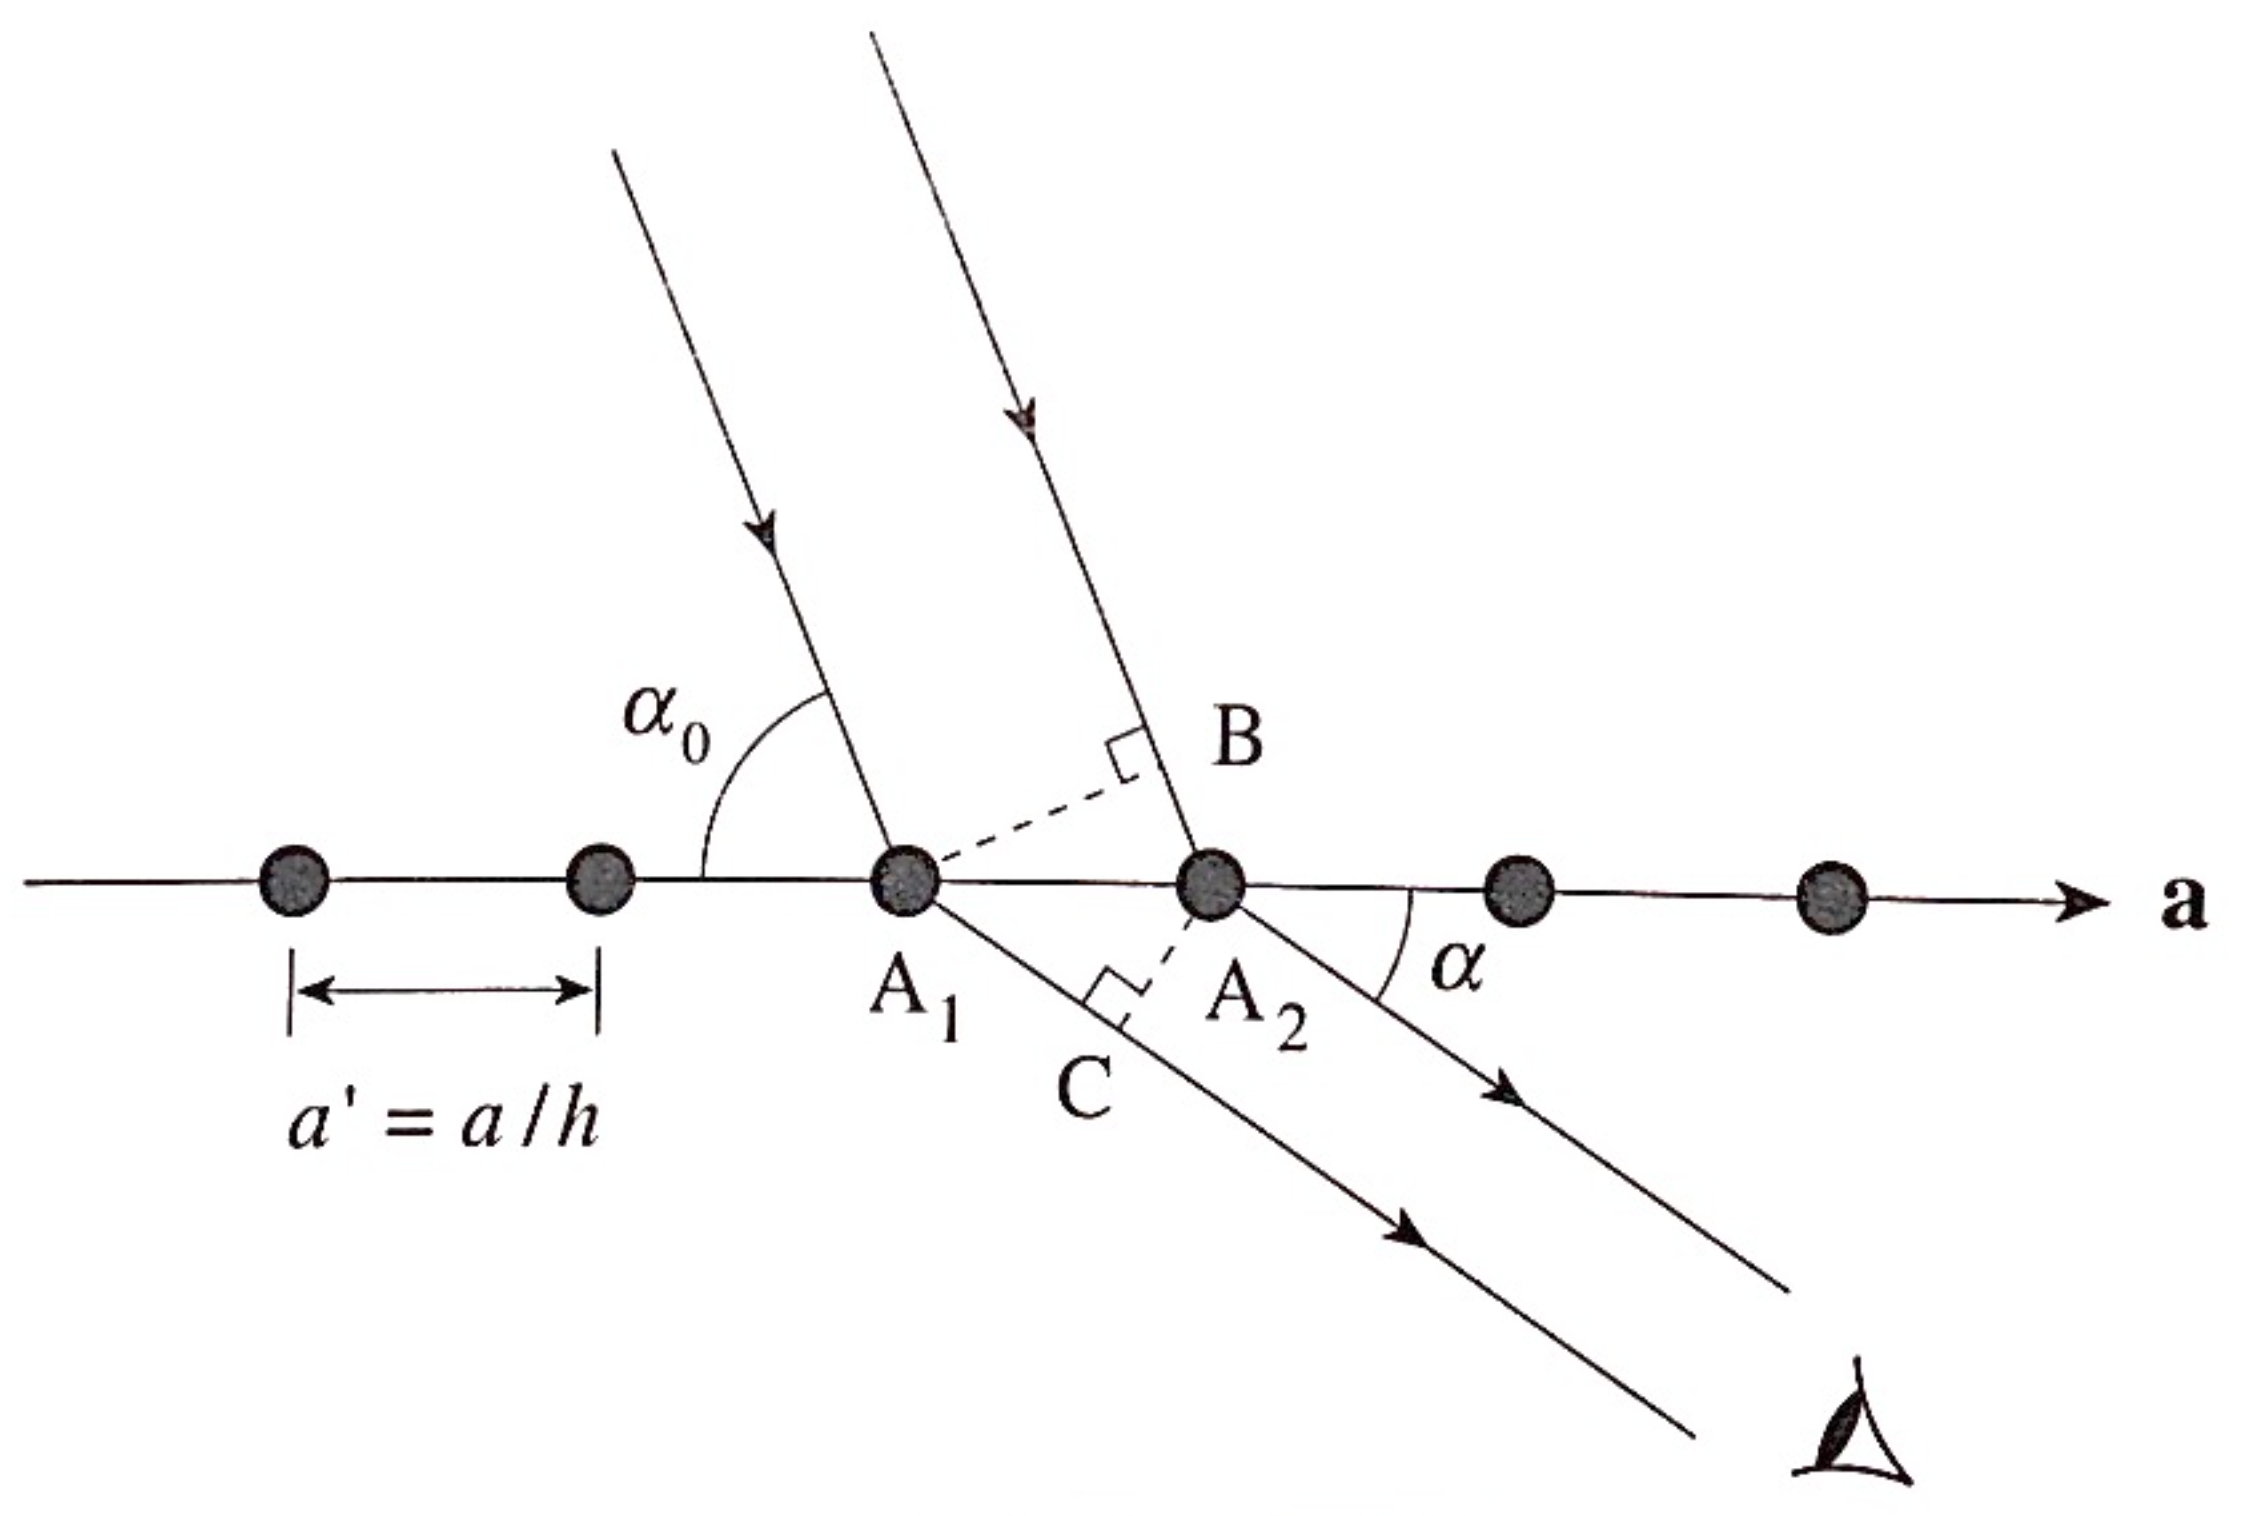
\includegraphics[width=0.45\linewidth]{../ExtFiles/vonLaueDerivation.png}
        \caption{Deriving the von Laue equations.}
        \label{fig:vonLaueDerivation}
    \end{figure}
    \begin{itemize}
        \item An X-ray diffraction pattern is a collection of spots of varying intensity.
        \begin{itemize}
            \item The arrangement of the spots provides a great deal of information on the crystal structure, as we will soon see.
        \end{itemize}
        \item We define
        \begin{equation*}
            \Delta = \overline{\text{A}_1\text{C}}-\overline{\text{A}_2\text{B}}
        \end{equation*}
        \begin{itemize}
            \item Imagine two parallel rays of light incident on points $\text{A}_1$ and $\text{A}_2$ in a crystal lattice.
            \item $\overline{\text{A}_1\text{C}}$ is the distance that the bottom beam travels after being scattered at $\text{A}_1$ and before the top beam is scattered at $\text{A}_2$.
            \item Symmetrically, $\overline{\text{A}_2\text{B}}$ is the distance that the top beam travels after the bottom beam is scattered at $\text{A}_2$ and before being scattered at $\text{A}_2$.
            \item Either way, $\Delta$ represents a kind of phase offset that occurs upon scattering. Say, for instance, that the two waves are in phase before scattering. Then from the perspective of the top wave, the bottom wave gets offset by $\Delta$ relative to it during the scattering process, and vice versa from the perspective of the bottom wave.
        \end{itemize}
        \item If the distance $\Delta$ is equal to an integral multiple of the wavelength of the X-ray radiation, the two diffracted beams will interfere constructively. Mathematically, since
        \begin{align*}
            \overline{\text{A}_1\text{C}} &= a'\cos\alpha&
            \overline{\text{A}_2\text{B}} &= a'\cos\alpha_0
        \end{align*}
        as we may readily read from Figure \ref{fig:vonLaueDerivation}, we require
        \begin{align*}
            n\lambda &= \Delta\\
            &= \overline{\text{A}_1\text{C}}-\overline{\text{A}_2\text{B}}\\
            &= a'(\cos\alpha-\cos\alpha_0)\\
            nh\lambda &= a(\cos\alpha-\cos\alpha_0)
        \end{align*}
    \end{itemize}
    \item \textbf{First-order reflection}: A diffraction spot that corresponds to $n=1$ in the above equation.
    \item \textbf{Second-order reflection}: A diffraction spot that corresponds to $n=2$ in the above equation.
    \item \textbf{$\bm{n}^\textbf{th}$-order reflection}: A diffraction spot that corresponds to $n$ in the above equation.
    \item \textbf{von Laue equations}: The following three equations, which relate the quantities involved in a first-order reflection. \emph{Given by}
    \begin{align*}
        a(\cos\alpha-\cos\alpha_0) &= h\lambda&
        b(\cos\beta-\cos\beta_0) &= k\lambda&
        c(\cos\gamma-\cos\gamma_0) &= l\lambda
    \end{align*}
    where $\alpha_0,\beta_0,\gamma_0$ are the angles of incidence of the X-ray radiation with respect to the \textbf{a}, \textbf{b}, and \textbf{c} axes of the crystal, respectively, and $\alpha$, $\beta$, and $\gamma$ are the corresponding diffraction angles.
    \item An example of how to use the von Laue equations.
    \begin{itemize}
        \item Consider the diffraction pattern obtained when an X-ray beam is directed at a crystal whose unit cell is primitive cubic.
        \item Orient the crystal such that the incident X-rays are perpendicular to the \textbf{a} axis of the crystal.
        \item Then the relevant von Laue equation reduces to $a\cos\alpha=h\lambda$.
        \item It follows that discrete angles will yield discrete spots?
    \end{itemize}
    \item A more general situation.
    \begin{itemize}
        \item For an arbitrary $hkl$ plane, the direction of diffraction with respect to the \textbf{a} axis is the same as that for the $h00$ planes. But there is also diffraction with respect to the \textbf{b} and \textbf{c} axes.
        \item The diffraction spots from an $hkl$ plane (with fixed $h$) will lie along the surface of a cone that makes an angle $\alpha$ with respect to the \textbf{a} axis of the crystal.
    \end{itemize}
    \item The Bragg diffraction.
    \begin{itemize}
        \item We have
        \begin{equation*}
            \lambda=2\left( \frac{d}{n} \right)\sin\theta
        \end{equation*}
        where $\theta$ is the angle of incidence (and reflection) of the X-rays with respect to the lattice plane, $\lambda$ is the wavelength of the X-ray radiation, and $n=1,2,\dots$ is the order of the reflection.
        \item $d$ in terms of the Miller indices for a cubic unit cell gives
        \begin{equation*}
            \sin^2\theta = \frac{n^2\lambda^2}{4a^2}(h^2+k^2+l^2)
        \end{equation*}
        \item Tian will not go through the details, but there will be a homework problem in which we will explore this.
    \end{itemize}
    \item Rotating the sample vs. rotating the incident beam in an X-ray diffraction experiment.
    \begin{itemize}
        \item In most cases, we fix the incident beam orientation and rotate the sample on the sample stage.
    \end{itemize}
    \item Midterms back today or tmw.
    \item The grade distribution in the course.
    \begin{itemize}
        \item A or A- is typically 65-70\%.
    \end{itemize}
\end{itemize}



\section{The Scattering Factor and Intensity}
\begin{itemize}
    \item \marginnote{5/18:}Reviews the Bragg diffraction.
    \begin{itemize}
        \item There is no such thing as a 222 or a 333 lattice plane; rather, there are 111 lattice planes with higher order diffractions.
        \item Tian says something about higher order reflections?
    \end{itemize}
    \item \textbf{Scattering factor} (of an atom): The following quantity, where $\rho(r)$ is the spherically symmetric electron density (number of electrons per unit volume) of the atom and $k=4\pi\sin(\theta)/\lambda$. In turn, $\theta$ is the scattering angle and $\lambda$ is the wavelength of the X-radiation. \emph{Denoted by} $\bm{f}$. \emph{Given by}
    \begin{equation*}
        f = 4\pi\int_0^\infty\rho(r)\frac{\sin kr}{kr}r^2\dd{r}
    \end{equation*}
    \begin{itemize}
        \item The integral $4\pi\int_0^\infty\rho(r)r^2\dd{r}$ gives the total number of electrons in the atom.
    \end{itemize}
    \item The total scattering intensity is related to the periodic structure of the electron density in the crystal.
    \begin{itemize}
        \item If the crystal is oriented such that the von Laue equation governing scattering from atoms along the $a$ axis is satisfied, then
        \begin{align*}
            \Delta_{11} &= \Delta_{22}
                = \frac{a}{h}(\cos\alpha-\cos\alpha_0)
                = \lambda&
            \Delta_{12} &= x(\cos\alpha-\cos\alpha_0)
        \end{align*}
        \item Combining these two equations, we learn that
        \begin{equation*}
            \Delta_{12} = \frac{\lambda hx}{a}
        \end{equation*}
        \item The difference in path length corresponds to a phase difference between the diffracted beams from successive 1 and 2 atoms of
        \begin{equation*}
            \phi = 2\pi\frac{\Delta_{12}}{\lambda}
            = 2\pi\frac{\lambda hx/a}{\lambda}
            = \frac{2\pi hx}{a}
        \end{equation*}
        \item The amplitude of the light scattered from successive 1 and 2 atoms is then
        \begin{align*}
            A &= f_1\cos\omega t+f_2\cos(\omega t+\phi)\\
            &= f_1\e[i\omega t]+f_2\e[i(\omega t+\phi)]
        \end{align*}
        \item The detected intensity is proportional to the square of the magnitude of the amplitude.
        \begin{align*}
            I \propto |A|^2 &= [f_1\e[i\omega t]+f_2\e[i(\omega t+\phi)]][f_1\e[-i\omega t]+f_2\e[-i(\omega t+\phi)]]\\
            &= f_1^2+f_1f_2\e[i\phi]+f_1f_2\e[-i\phi]+f_2^2\\
            &= f_1^2+f_2^2+2f_1f_2\cos\phi
        \end{align*}
        \begin{itemize}
            \item The first two terms reflect the constructive interference of the X-rays scattered from the set of parallel planes through the 1 atoms and 2 atoms, respectively.
            \item The third term takes into account the interference of the scattering from these two sets of parallel planes.
        \end{itemize}
        \item We can therefore ignore the $\e[i\omega t]$ term and define
        \begin{equation*}
            F(h) = f_1+f_2\e[i\phi]
            = f_1+f_2\e[2\pi ihx/a]
        \end{equation*}
        \item The intensity is then proportional to $|F(h)|^2$.
        \item Generalizing to three dimensions for a unit cell that contains atoms of type $j$ located at points $x_j,y_j,z_j$ gives
        \begin{equation*}
            F(hkl) = \sum_jf_j\e[2\pi i(hx_j/a+ky_j/b+lz_j/c)]
            = \sum_jf_j\e[2\pi i(hx_j'+ky_j'+lz_j')]
        \end{equation*}
        where $x_j'=x_j/a$, $y_j'=y_j/b$, and $z_j'=z_j/c$.
    \end{itemize}
    \item An analysis of the \ce{CsCl} body-centered cubic lattice, where we take the unit cell to have eighth chloride atoms at every corner and one cesium ion in the center.
    \begin{itemize}
        \item Taking $f_+$ to be the scattering factor of the \ce{Cs+} cations and $f_-$ to be the scattering factor of the \ce{Cl-} anions, we get
        \begin{align*}
            F(hkl) &= 1\times f_-\e[\pi i(h+k+l)]+\frac{1}{8}\times f_+\left[ \e[0]+\e[2\pi ih]+\e[2\pi ik]+\e[2\pi il]+\e[2\pi i(h+k)]+\e[2\pi i(k+l)]+\e[2\pi i(h+l)]+\e[2\pi i(h+k+l)] \right]\\
            &= f_-(-1)^{h+k+l}+\frac{1}{8}f_+[8]\\
            &=
            \begin{cases}
                f_++f_- & h+k+l\text{ is even}\\
                f_+-f_- & h+k+l\text{ is odd}
            \end{cases}
        \end{align*}
        where we substitute $\e[\pi i]=-1$ and $\e[2\pi i]=1$ to get from the first line to the second.
    \end{itemize}
\end{itemize}



\section{Continuous Structure Factors and Adsorption}
\begin{itemize}
    \item \marginnote{5/20:}More on the \ce{CsCl} example today.
    \begin{itemize}
        \item We simplify $\e[i\pi(h+k+l)]$ to $(-1)^{h+k+l}$ by expanding to $\cis[\pi(h+k+l)]$, ignoring the imaginary part to get $\cos[\pi(h+k+l)]$, the sign of which does depend on whether the natural number $h+k+l$ is even or odd exactly like $(-1)^{h+k+l}$.
    \end{itemize}
    \item \ce{CsI} example.
    \begin{itemize}
        \item \ce{Cs+} and \ce{I-} are \textbf{isoelectronic}.
        \item We have that
        \begin{equation*}
            f_+(\ce{Cs+}) = f_-(\ce{I-})
        \end{equation*}
    \end{itemize}
    \item The structure factor and the electron density are related by a Fourier transform.
    \begin{itemize}
        \item In both atomic and molecular crystals, the electron density is not localized at individual points within the unit cell.
        \item We should consider the unit cell of the crystal to have a continuous electron density distribution $\rho(x,y,z)$.
        \item The structure factor is no longer simply a sum over discrete atoms but now becomes an integral over the continuous electron density distribution in the unit cell, as follows.
        \begin{equation*}
            F(hkl) = \int_0^a\int_0^b\int_0^c\rho(x,y,z)\e[2\pi i(hx/a+ky/b+lz/c)]\dd{x}\dd{y}\dd{z}
        \end{equation*}
        \item For the entire crystal, we have the following.
        \begin{equation*}
            F(hkl) \propto \int_{-\infty}^\infty\int_{-\infty}^\infty\int_{-\infty}^\infty\rho(x,y,z)\e[2\pi i(hx/a+ky/b+lz/c)]\dd{x}\dd{y}\dd{z}
        \end{equation*}
        \item $F(hkl)$ is related to $\rho(x,y,z)$ by a \textbf{Fourier transform}.
        \begin{equation*}
            \rho(x,y,z) = \sum_{h=-\infty}^\infty\sum_{k=-\infty}^\infty\sum_{l=-\infty}^\infty F(hkl)\e[-2\pi i(hx/a+ky/b+lz/c)]
        \end{equation*}
        \item If we let $F(hkl)=A(hkl)+iB(hkl)$, then it follows that the intensity is
        \begin{equation*}
            I(hkl) \propto |F(hkl)|^2 = [A(hkl)]^2+[B(hkl)]^2
        \end{equation*}
    \end{itemize}
    \item An electron-density map of a benzoic acid molecule.
    \begin{figure}[h!]
        \centering
        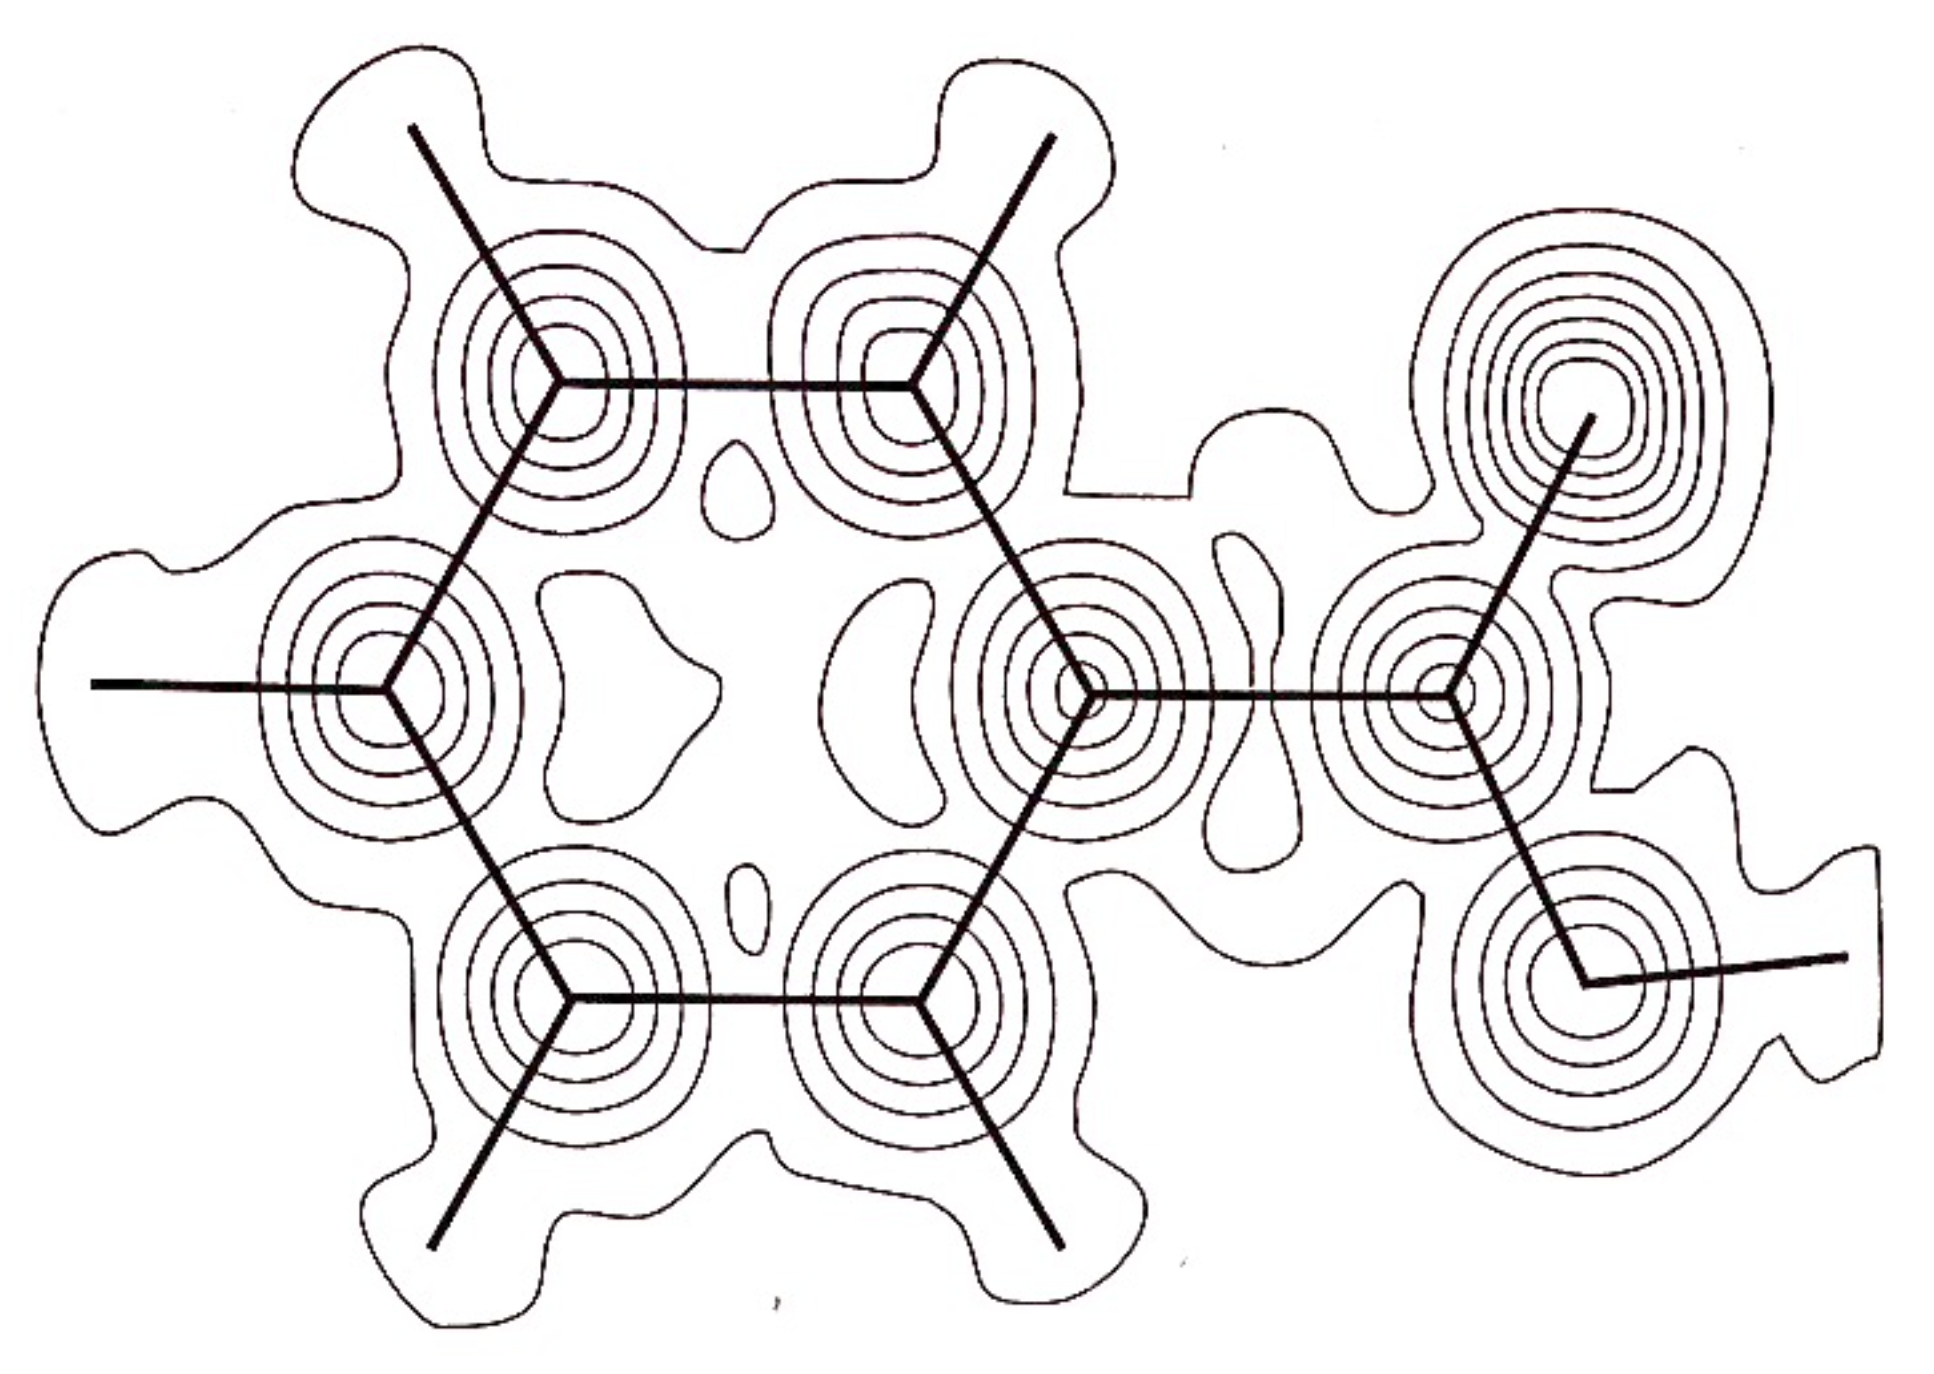
\includegraphics[width=0.4\linewidth]{../ExtFiles/benzoicAcidEdensity.png}
        \caption{The electron density of benzoic acid.}
        \label{fig:benzoicAcidEdensity}
    \end{figure}
    \begin{itemize}
        \item An electron-density map of a benzoic acid molecule determined from the X-ray diffraction pattern of a benzoic acid crystal.
        \item Each contour line corresponds to a constant value of the electron density.
        \item The location of the nuclei are readily deduced from this electron-density map and are represented by the vertices of the solid lines.
    \end{itemize}
    \item A gas molecule can physisorb or chemisorb to a solid surface.
    \begin{figure}[h!]
        \centering
        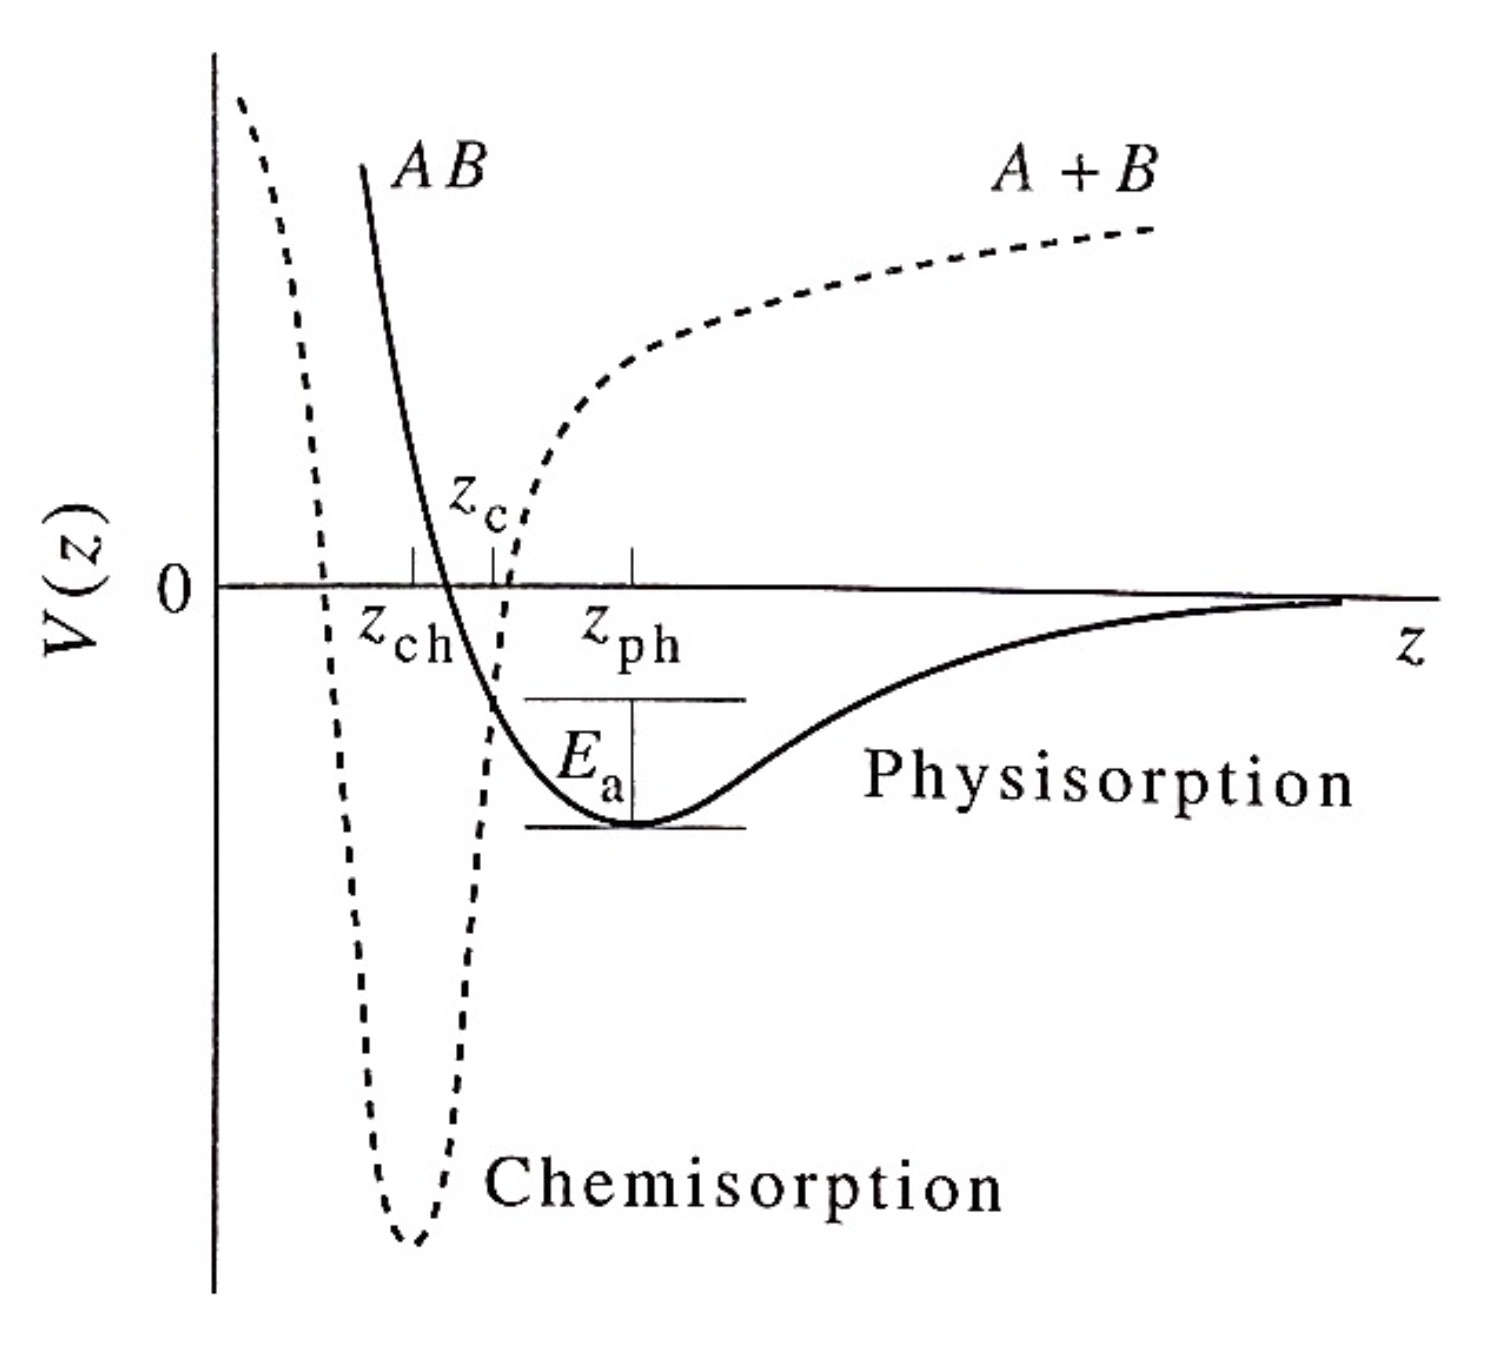
\includegraphics[width=0.36\linewidth]{../ExtFiles/PhysiChemiSorption.png}
        \caption{Comparing physisorption and chemisorption.}
        \label{fig:PhysiChemiSorption}
    \end{figure}
    \begin{itemize}
        \item Figure \ref{fig:PhysiChemiSorption} shows one-dimensional potential-energy curves for the physisorption of molecule \ce{AB} (solid line) and the dissociative chemisorption of \ce{AB} (dashed line).
        \item The quantity $z$ is the distance from the surface.
        \item In the physisorbed state, the molecule \ce{AB} is bound to the surface by van der Waals forces.
        \item In the chemisorbed state, the \ce{A-B} bond is broken, and the individual atoms are bound covalently or ionically on the surface.
        \begin{itemize}
            \item As such, chemisorbed molecules are bound more strongly, are held closer to the surface.
            \item As $z\to\infty$, $V$ approaches a value greater than zero because \ce{AB} is dissociated here. The asymptote is the bond dissociation energy (BDE).
            \item Additionally, while \ce{A + B} may be at zero, what we have here is \ce{A+ + B-}. As such, we have the Coulomb potential, and the charged ions are unstable to be apart.
        \end{itemize}
        \item The points $z_\text{ch}$ and $z_\text{ph}$ are the surface-molecule bond lengths for a chemisorbed and physisorbed molecule, respectively. The length of the substrate-adsorbate bond is shorter for a chemisorbed molecule than for a physisorbed molecule.
        \item The two potential curves cross at $z_c$. The activation energy for the conversion from physisorption to chemisorption is measured from the bottom of the physisorbed potential and is $E_a$.
    \end{itemize}
    \item \textbf{Adsorption isotherm}: A plot of surface coverage as a function of gas pressure at constant temperature.
    \item Langmuir's assumptions.
    \begin{itemize}
        \item The adsorbed molecules do not interact with one another.
        \item The enthalpy of adsorption was independent of surface coverage.
        \item There are a finite number of surface sites where a molecule can adsorb.
        \item The process of adsorption and desorption is depicted by the reversible elementary process
        \begin{equation*}
            \ce{A(g) + S(s)} \Longleftrightarrows[k_a][k_d] \ce{A-S(s)}
        \end{equation*}
        with equilibrium constant
        \begin{equation*}
            K_c = \frac{k_a}{k_d}
            = \frac{\cnc{A-S}}{\cnc{A}\cnc{S}}
        \end{equation*}
        where $k_a$ and $k_d$ are the rate constants for \underline{a}dsorption and \underline{d}esorption, respectively.
    \end{itemize}
    \item The fact that $k_a$ and $k_d$ are constants independent of the extent of surface coverage implies that adsorbed molecules do not interact with one another.
    \item An analysis of surface coverage.
    \begin{itemize}
        \item Let $\sigma_0$ be the concentration of surface sites in units of \si{\per\meter\squared}.
        \item If the fraction of surface sites occupied by an adsorbate is $\theta$, then $\sigma$ (the adsorbate concentration on the surface) is $\theta\sigma_0$ and the concentration of empty surface sites is give by $\sigma_0-\theta\sigma_0=(1-\theta)\sigma_0$.
        \item We have that
        \begin{align*}
            v_d &= k_d\theta\sigma_0&
            v_a &= k_a(1-\theta)\sigma_0\cnc{A}
        \end{align*}
        where $v_d$ is the rate of desorption, $v_a$ is the rate of absorption, and $\cnc{A}$ is the number density or the concentration of \ce{A(g)}.
        \item It follows that at equilibrium,
        \begin{align*}
            k_d\theta &= k_a(1-\theta)\cnc{A}\\
            \frac{1}{\theta} &= 1+\frac{1}{K_c\cnc{A}}
        \end{align*}
        \item Additionally, since
        \begin{align*}
            \cnc{A} = \frac{P_{\ce{A}}}{\kB T}
        \end{align*}
        the Langmuir adsorption isotherm is
        \begin{equation*}
            \frac{1}{\theta} = 1+\frac{1}{bP_{\ce{A}}}
        \end{equation*}
        where we have defined $b=K_c/\kB T$.
    \end{itemize}
    \item For different materials, the same mass may correspond to orders of magnitude different surface areas (consider MOFs for instance).
    \item Langmuir adsorption isotherm for the case in which a diatomic molecule dissociates upon adsorption to the surface.
    \begin{itemize}
        \item This reaction can be written as
        \begin{align*}
            \ce{A2(g) + 2S(s)} &\Longleftrightarrows[k_a][k_d] \ce{2A-S(s)}&
            K_c &= \frac{k_a}{k_d}
                = \frac{\cnc{A-S}^2}{\cnc{A2}\cnc{S}^2}
        \end{align*}
        \item Two surface sites are involved in the adsorption and desorption process.
        \begin{align*}
            v_a &= k_a\cnc{A2}(1-\theta)^2\sigma_0^2&
            v_d &= k_d\theta^2\sigma_0^2
        \end{align*}
        \item At equilibrium, these rates are equal, i.e.,
        \begin{align*}
            k_a\cnc{A2}(1-\theta)^2 &= k_d\theta^2\\
            \theta &= \frac{K_c^{1/2}\cnc{A2}^{1/2}}{1+K_c^{1/2}\cnc{A2}^{1/2}}
        \end{align*}
        \item Having defined $\cnc{A}=P_{\ce{A}}/\kB T$ and $b=K_c/\kB T$, we have
        \begin{align*}
            \theta &= \frac{b_{\ce{A2}}^{1/2}P_{\ce{A2}}^{1/2}}{1+b_{\ce{A2}}^{1/2}P_{\ce{A2}}^{1/2}}\\
            \frac{1}{\theta} &= 1+\frac{1}{b_{\ce{A2}}^{1/2}P_{\ce{A2}}^{1/2}}
        \end{align*}
    \end{itemize}
\end{itemize}



\section{Office Hours (Tian)}
\begin{itemize}
    \item The whole $F\propto\sigma\rho$ thing from Lecture 4.
    \item The presence of lack thereof of the $1/2$ coefficient in $Z_{\ce{A}\ce{A}}$ and $Z_{\ce{A}\ce{B}}$.
    \item Lecture 13 example problems.
    \begin{itemize}
        \item Equilibrium constants appear in reversible reactions.
        \item Only applicable for reversible elementary steps.
        \item If there's a problem that involves equilibrium constants, he will identify it; tell us that a reaction is reversible and equilibrium constants need to be considered.
    \end{itemize}
    \item Will there be extra office hours before the final?
    \item Midterm info.
    \begin{itemize}
        \item The midterm had a bimodal (2 peaks) distribution.
    \end{itemize}
    \item Miller indices.
    \begin{itemize}
        \item We define 100 planes by convention.
        \item The middle plane in Figure 31.9a intersects the $a$-axis at $(1,0,0)$, and never intersects the $b$ or $c$ axes. However, we can conceptually define an intersection at $\infty$, leading to $k=b/\infty=0$ and similarly for $l$.
    \end{itemize}
    \item Final info.
    \begin{itemize}
        \item Homeworks 5-6 for the computation problem.
        \item Rest are true/false and conceptual (like defining the Miller indices, for example).
        \item Open note, calculator, but not open internet.
        \item We can bring our computer for online notes, but we cannot search anything.
        \item Only conceptual problems on X-ray diffraction.
        \item No class on Friday Week 9.
    \end{itemize}
    \item X-ray diffraction info.
    \begin{itemize}
        \item Some people who have taken Advanced Inorgo will have already seen this, but it's the first time for most people.
    \end{itemize}
\end{itemize}



\section{Chapter 31: Solids and Surface Chemistry}
\emph{From \textcite{bib:McQuarrieSimon}.}
\begin{itemize}
    \item \marginnote{5/24:}The experimental setup for X-ray diffraction.
    \begin{itemize}
        \item Generating X-rays.
        \begin{itemize}
            \item A metal target (often copper) is bombarded with high-energy electrons inside a vacuum tube.
            \item This bombardment generates electronically excited copper cations which relax back to their ground state by emitting a photon.
            \item A copper sample generates two types of photons: One with $\lambda=\SI{154.433}{\pico\meter}$ and another with $\lambda=\SI{154.051}{\pico\meter}$.
        \end{itemize}
        \item One of these two wavelengths is directed at a single sample crystal.
        \item The crystal is located on a rotatable mount, enabling the scientist to orient the incident X-rays with respect to the three crystallographic axes.
        \item Most radiation passes through a given crystal, but a little bit is diffracted, giving rise to the \textbf{diffraction pattern}.
    \end{itemize}
    \item \textbf{Diffraction pattern}: The image recorded on the detector, where dark spots correspond to concentrated diffracted X-rays.
    \item The positions and intensities of the diffraction spots are determined by the spacing between the different sets of parallel $hkl$ planes of the crystal lattice.
    \item Comments on Figure \ref{fig:vonLaueDerivation}.
    \begin{itemize}
        \item Lattice points $\text{A}_1,\text{A}_2$ lie in neighboring $hkl$ planes along the \textbf{a} axis of the crystal and are separated by $a'$.
        \item $\alpha_0$ is the angle of incidence of the X-ray beam.
        \item $\alpha$ is the angle of diffraction of the X-ray beam.
        \item $\Delta$ is the difference in path length of the X-rays diffracted at lattice points $\text{A}_1,\text{A}_2$ by the time they reach the observer (or collection sheet).
        \item "If we extend [our discussion of constructive and destructive interference] to include diffraction from all the atoms in the row shown in [Figure \ref{fig:vonLaueDerivation}], then to observe a diffraction signal, the light diffracted from each atom in the row must interfere constructively. This means that the crystal plane must be oriented with respect to the incident X-rays so that $\Delta$ is equal to an integral multiple of the wavelength of the X-ray radiation" \parencite[1283]{bib:McQuarrieSimon}.
        \item The substitution $a'=a/h$ allows us to write the diffraction equation in terms of the Miller index and the unit cell length.
    \end{itemize}
    \item Describing the diffraction pattern generated by the first-order reflections of the $h00$ planes in a primitive cubic crystal that is oriented such that the incident X-rays are perpendicular to the \textbf{a} axis of the crystal.
    \begin{figure}[h!]
        \centering
        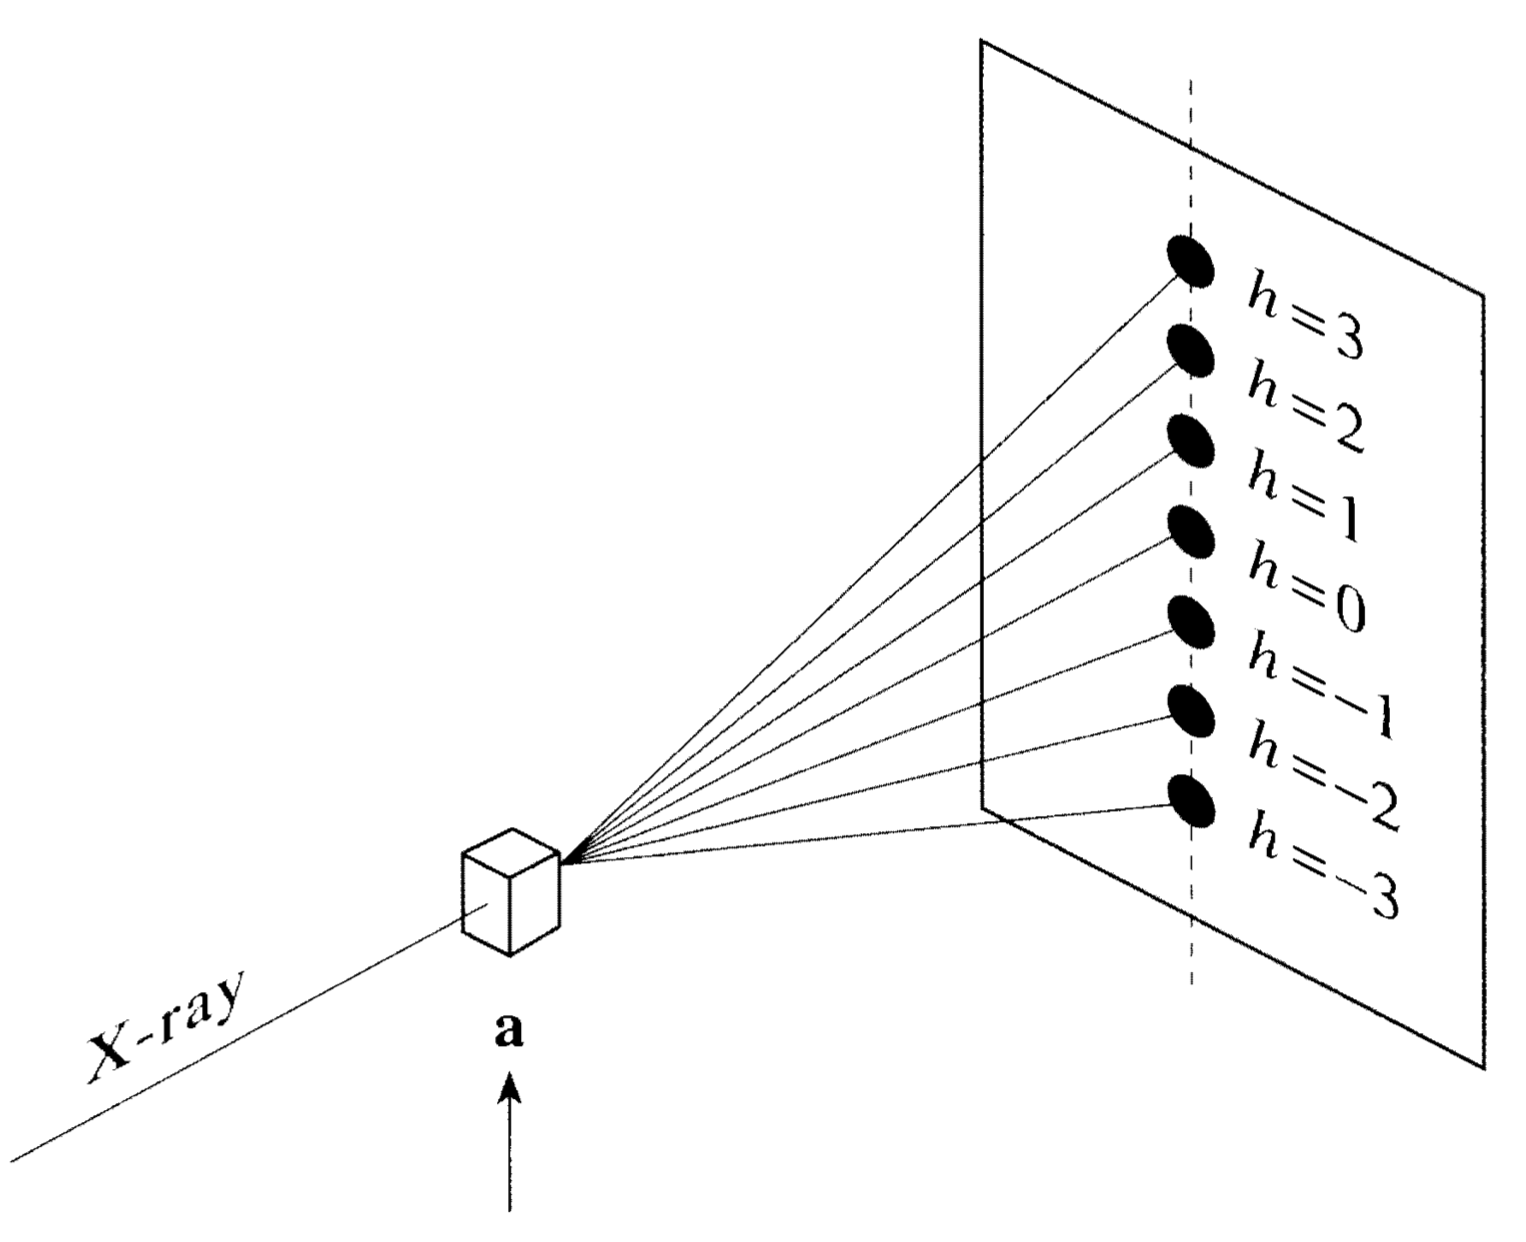
\includegraphics[width=0.4\linewidth]{../ExtFiles/primitiveDiff.png}
        \caption{The diffraction pattern of the $h00$ planes in a primitive cubic crystal.}
        \label{fig:primitiveDiff}
    \end{figure}
    \begin{itemize}
        \item The perpendicular orientation tells us that $\alpha_0=\ang{90}$.
        \item Thus, the von Laue equations become
        \begin{align*}
            a\cos\alpha &= h\lambda\\
            b(\cos\beta-\cos\beta_0) &= k\lambda\\
            c(\cos\gamma-\cos\gamma_0) &= l\lambda
        \end{align*}
        \item The first equation says that each value of $h$ (i.e., each incremental plane spacing) corresponds to a specific scattering angle $\alpha$.
        \begin{itemize}
            \item For $h=0$, we have $\cos\alpha=0$ and thus $\alpha=\ang{90}$.
            \item For $h=1$, we have $\cos\alpha=\lambda/a$.
            \item For $h=2$, we have $\cos\alpha=2\lambda/a$.
            \item And on and on.
        \end{itemize}
        \item Since $k,l=0$ in all of these planes, the second and third equations say, respectively, that $\beta=\beta_0$ and $\gamma=\gamma_0$.
        \item Thus, we obtain the diffraction pattern in Figure \ref{fig:primitiveDiff}.
    \end{itemize}
    \item Example: Calculating the spacing between lattice points along the \textbf{a} axis in a primitive cubic crystal from the first-order reflections of the $000$ and $100$ planes.
    \begin{figure}[h!]
        \centering
        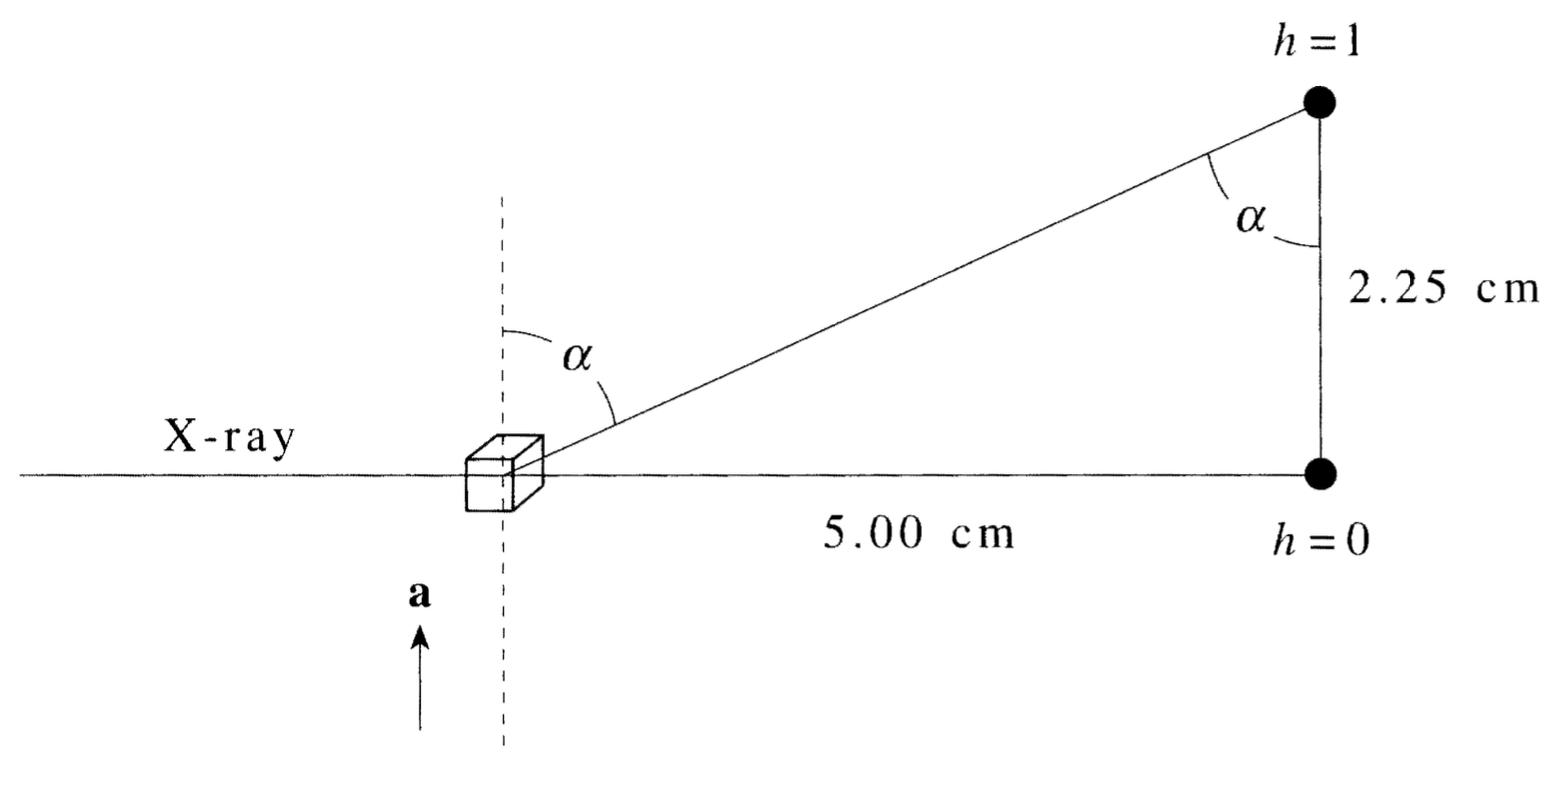
\includegraphics[width=0.55\linewidth]{../ExtFiles/primitiveLatticeSpace.png}
        \caption{Primitive cubic lattice spacing.}
        \label{fig:primitiveLatticeSpace}
    \end{figure}
    \begin{itemize}
        \item In our experimental setup, we use the $\lambda=\SI{154.433}{\pico\meter}$ line of copper as an X-ray source.
        \item We want to find $a$. We know that $a\cos\alpha=\lambda$. We also know that $\tan\alpha=5.00/2.25$. Therefore,
        \begin{equation*}
            a = \frac{\lambda}{\cos\left( \tan^{-1}(5.00/2.5) \right)}
            = \SI{376.37}{\pico\meter}
        \end{equation*}
    \end{itemize}
    \item Arbitrary $hkl$ planes.
    \begin{figure}[h!]
        \centering
        \begin{subfigure}[b]{0.49\linewidth}
            \centering
            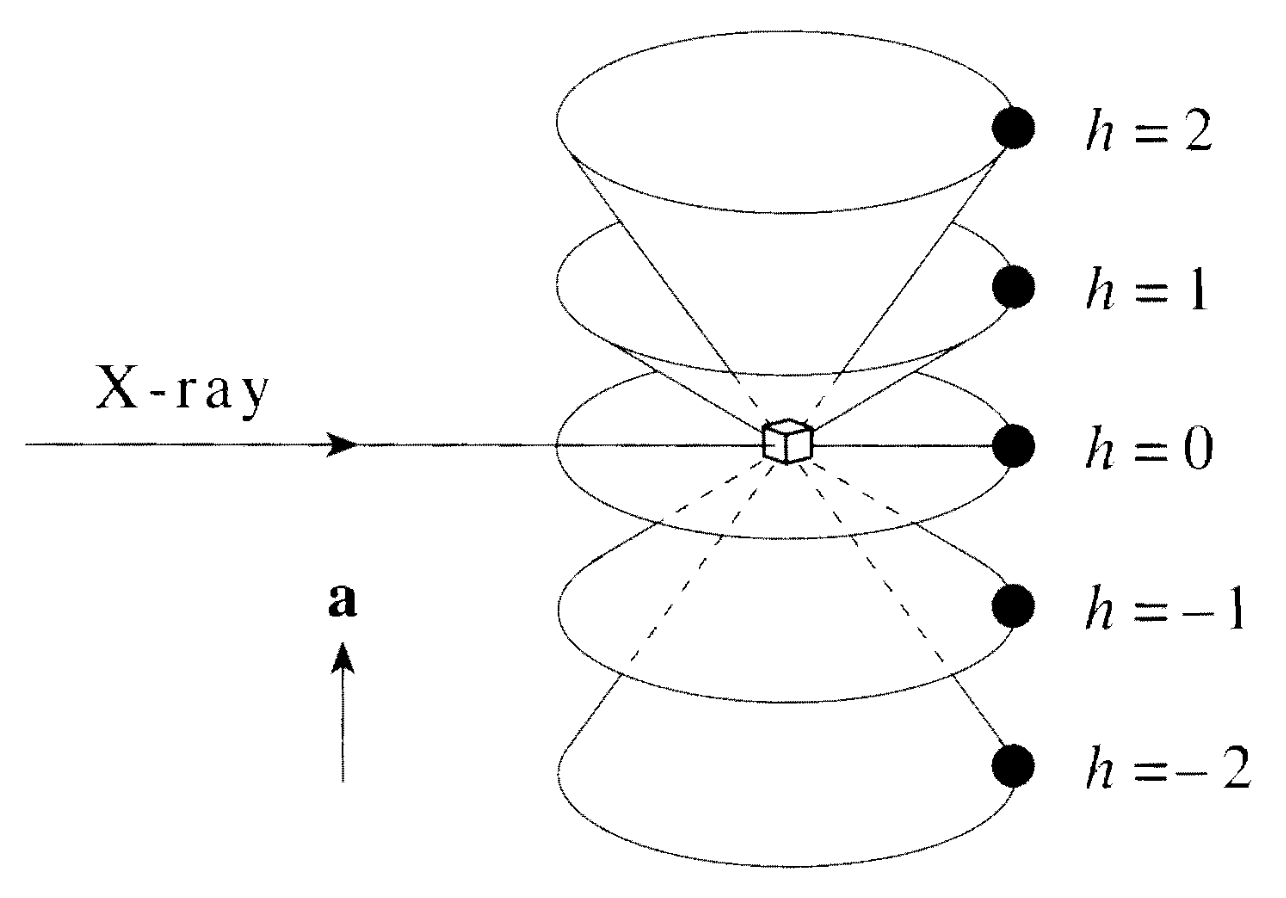
\includegraphics[width=0.71\linewidth]{../ExtFiles/primitiveDiffHKLa.png}
            \caption{General cone.}
            \label{fig:primitiveDiffHKLa}
        \end{subfigure}
        \begin{subfigure}[b]{0.49\linewidth}
            \centering
            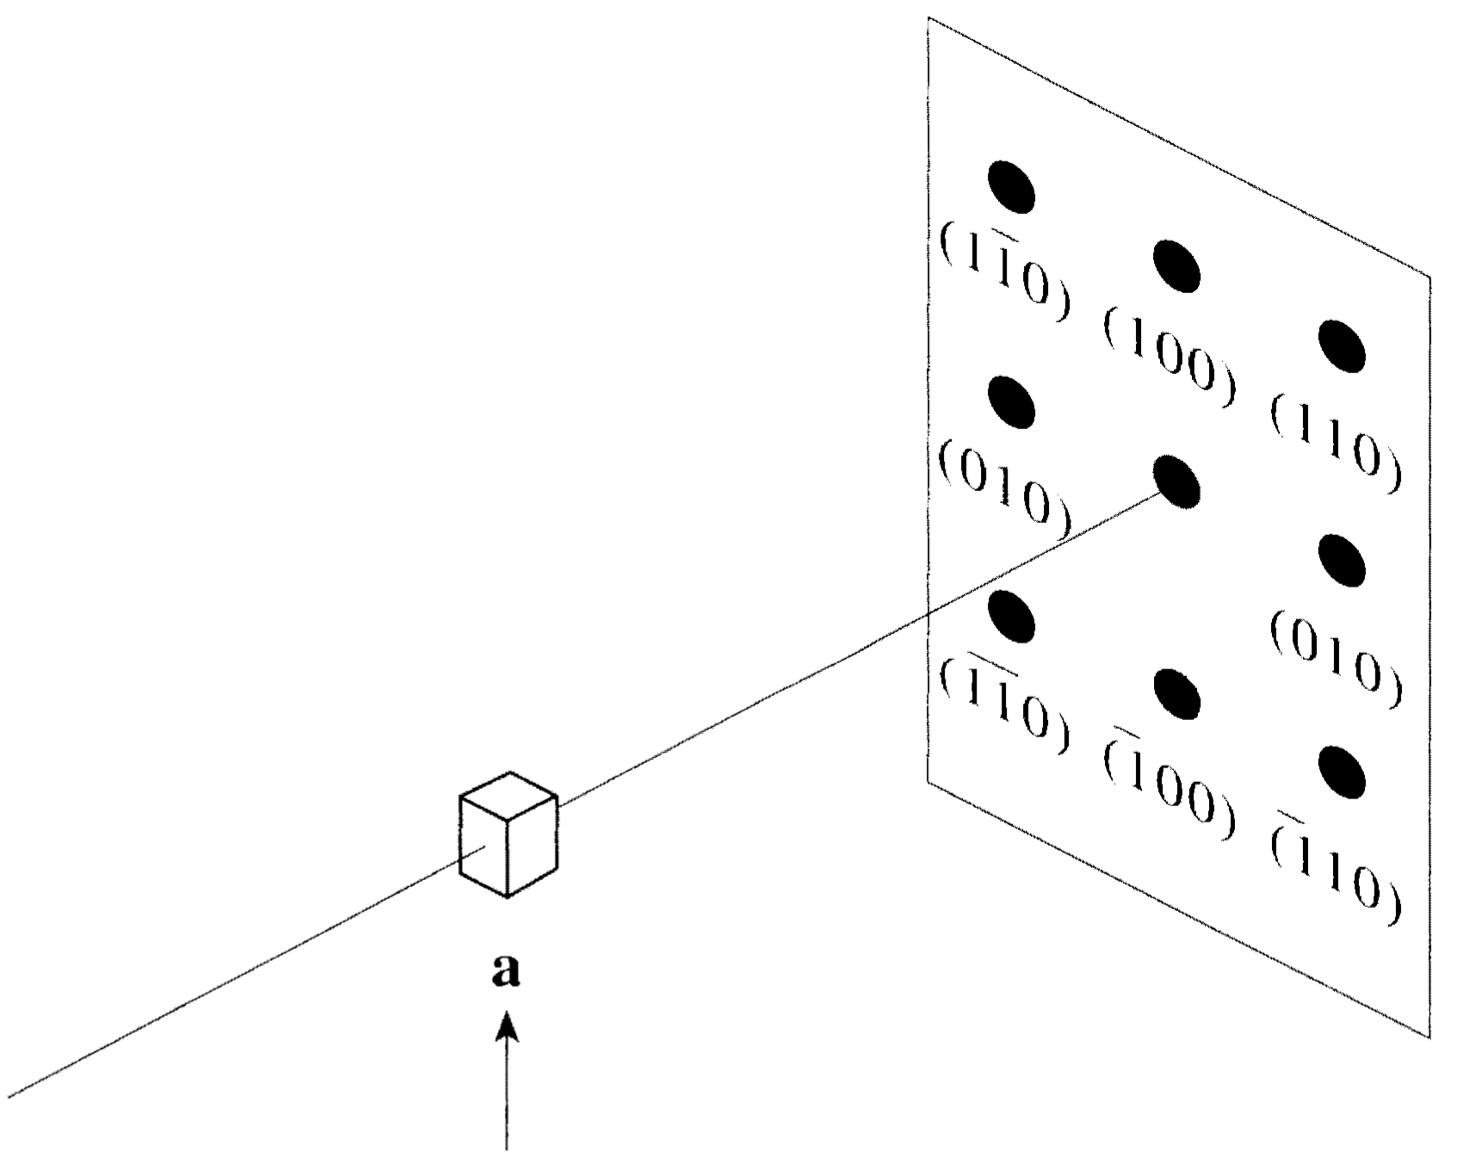
\includegraphics[width=0.77\linewidth]{../ExtFiles/primitiveDiffHKLb.png}
            \caption{Specific examples.}
            \label{fig:primitiveDiffHKLb}
        \end{subfigure}
        \caption{The diffraction pattern of the $hkl$ planes in a primitive cubic crystal.}
        \label{fig:primitiveDiffHKL}
    \end{figure}
    \begin{itemize}
        \item The direction of diffraction with respect to the \textbf{a} axis is the same as that for $h00$ planes, but there is also componentwise diffraction with respect to the \textbf{b} and \textbf{c} axes.
        \item Thus, the diffraction spots lie along the surface of a cone (see Figure \ref{fig:primitiveDiffHKLa}) that makes an angle $\alpha$ with respect to the incident X-ray beam in the plane defined by the X-ray beam and the \textbf{a} axis (i.e., the plane of the page in Figure \ref{fig:primitiveLatticeSpace}).
        \item Where exactly these spots lie depends on the other two von Laue equations.
        \item Some examples of spots corresponding to $hkl$ planes are given in Figure \ref{fig:primitiveDiffHKLb}.
    \end{itemize}
    \item Bragg's approach to diffraction.
    \begin{itemize}
        \item William Bragg (an English chemist) "modeled the diffraction of X-rays from crystals as originating from the reflection of X-rays from the various sets of parallel $hkl$ lattice planes" \parencite[1286-87]{bib:McQuarrieSimon}.
        \item The Bragg equation is
        \begin{equation*}
            \lambda = 2\left( \frac{d}{n} \right)\sin\theta
        \end{equation*}
        where $\theta$ is the angle of incidence (and reflection) of the X-rays with respect to the lattice plane, $\lambda$ is the wavelength of the X-rays, $n=1,2,\dots$ is the order of the reflection, and $d$ is the lattice plane spacing.
        \begin{itemize}
            \item For Bragg's derivation, see Problem \ref{prb:31-29}.
        \end{itemize}
        \item By squaring the above and substituting for $d^2$ the lattice plane spacing for a cubic unit cell, we obtain
        \begin{equation*}
            \sin^2\theta = \frac{n^2\lambda^2}{4a^2}(h^2+k^2+l^2)
        \end{equation*}
        \item Bragg's equation can be derived from the von Laue equations and vice versa (see Problems \ref{prb:31-44} and \ref{prb:31-45}), so the two formulations are equivalent.
    \end{itemize}
    \item In practice, diffraction spots are not observed from all $hkl$ planes and the intensity can vary significantly as well.
    \begin{itemize}
        \item "For example, an atomic crystal whose unit cell is body-centered cubic shows no diffraction from the $hkl$ planes in which $h+k+l$ is an odd number" \parencite[1287]{bib:McQuarrieSimon}.
        \item The key to understanding what determines the intensity of a diffraction spot lies in the details of how atoms diffract X-rays.
    \end{itemize}
    \item X-rays are scattered by the electrons in an atom, but since different atoms have different sized orbitals filled by different numbers of electrons, the scattering efficiency varies atom to atom. Hence we define the \textbf{scattering factor}.
    \item \textbf{Scattering factor} (of an atom): The following quantity, where $\rho(r)$ is the spherically symmetric electron density (number of electrons per unit volume) of the atom and $k=(4\pi/\lambda)\sin(\theta)$. In turn, $\theta$ is the scattering angle and $\lambda$ is the wavelength of the X-radiation. \emph{Denoted by} $\bm{f}$. \emph{Given by}
    \begin{equation*}
        f = 4\pi\int_0^\infty\rho(r)\frac{\sin kr}{kr}r^2\dd{r}
    \end{equation*}
    \begin{itemize}
        \item Wavelengths of X-rays are comparable in size to an atom, so the scatterings from different regions interfere with each other. The integrand accounts for this interference with the $\sin(kr)/kr$ term.
        \item The scattering factor increases as the number of electrons ($\rho(r)$) increases, and decreases as the angle of diffraction $\theta$ increases.
        \item The scattering factor for the case where $\theta=\ang{0}$ reduces to the total number of electrons in the atom or ion.
    \end{itemize}
    \item Deriving an expression for the scattering intensity.
    \begin{figure}[h!]
        \centering
        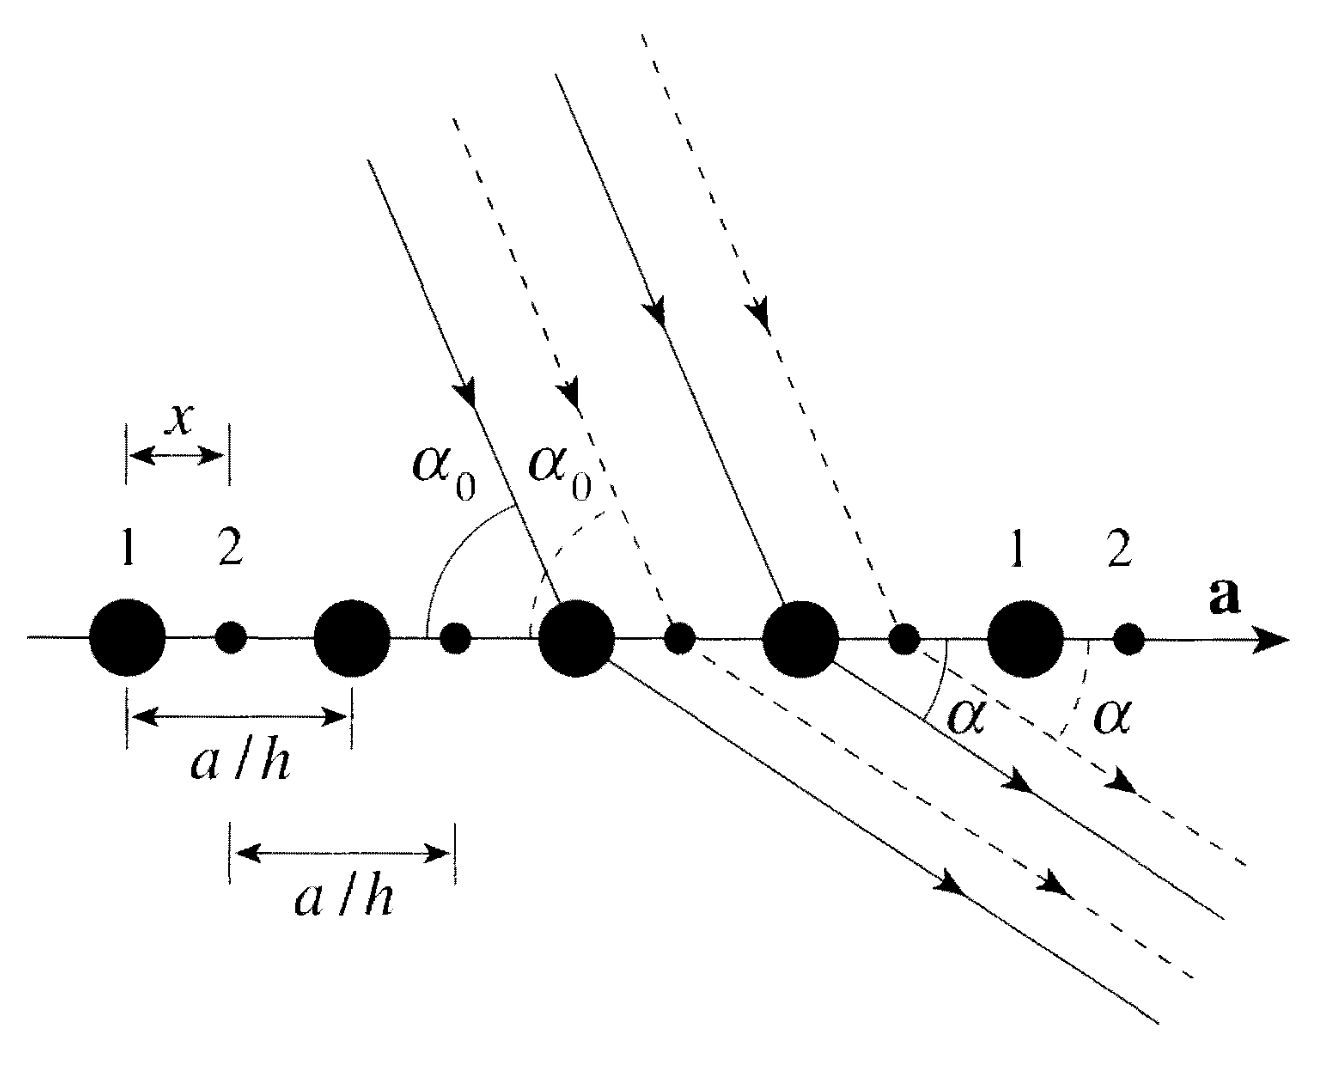
\includegraphics[width=0.37\linewidth]{../ExtFiles/2atomScattering.png}
        \caption{The scattering from a lattice consisting of two types of atoms.}
        \label{fig:2atomScattering}
    \end{figure}
    \begin{itemize}
        \item Consider a one-dimensional lattice consisting of two different types of atoms, 1 and 2. Let these atoms have scattering factors $f_1,f_2$, respectively.
        \item The differences $\Delta_{11}$ and $\Delta_{22}$ in path length traveled by X-rays diffracted by successive 1 atoms and 2 atoms, respectively, and corresponding to first-order reflections are equal and given by the following, as can easily be determined from Figure \ref{fig:2atomScattering} and the von Laue equations.
        \begin{equation*}
            \Delta_{11} = \Delta_{22}
            = \frac{a}{h}(\cos\alpha-\cos\alpha_0)
            = \lambda
        \end{equation*}
        \item Similarly, the difference $\Delta_{12}$ in path length traveled by X-rays diffracted by consecutive 1 and 2 atoms and corresponding to a first-order reflection is given by the following and is not equal to an integral number of wavelengths.
        \begin{equation*}
            \Delta_{12} = x(\cos\alpha-\cos\alpha_0)
        \end{equation*}
        \item An alternate form for $\Delta_{12}$ can be obtained by solving the expression for $\Delta_{11}=\Delta_{22}$ for $\cos\alpha-\cos\alpha_0$ and substituting into the above equation to yield
        \begin{equation*}
            \Delta_{12} = \frac{\lambda hx}{a}
        \end{equation*}
        \item This difference in path length corresponds to a phase offset
        \begin{equation*}
            \phi = 2\pi\frac{\Delta_{12}}{\lambda}
            = 2\pi\frac{\lambda hx/a}{\lambda}
            = \frac{2\pi hx}{a}
        \end{equation*}
        \begin{itemize}
            \item Note that to derive this expression, we first take the difference in path length and divide by $\lambda$ to determine the phase offset in "number of waves." We then multiply by $2\pi$ to convert to radians.
            \item For instance, if $\Delta_{12}=1.5\lambda$, then $\Delta_{12}/\lambda=1.5\,\text{waves}=3\pi\,\text{radians}$, as should make intuitive sense.
        \end{itemize}
        \item It follows that the total amplitude of the light scattered from successive 1 and 2 atoms is
        \begin{equation*}
            A = f_1\cos\omega t+f_2\cos(\omega t+\phi)
        \end{equation*}
        \begin{itemize}
            \item Technically, what's given is a wave function in terms of time $t$.
            \item Also note that the left term in the above expression gives the contribution of the light scattered by successive 1 atoms and the right term gives the contribution of the light scattered by successive 2 atoms. By the superposition principle, the total wave function is the sum of the two partial wave functions, as we have above.
        \end{itemize}
        \item For convenience, we may switch the above expression to exponential notation.
        \begin{equation*}
            A = f_1\e[i\omega t]+f_2\e[i(\omega t+\phi)]
            = \left( f_1+f_2\e[i\phi] \right)\e[i\omega t]
        \end{equation*}
        \item Since the intensity of electromagnetic waves is proportional to the square of the magnitude of the amplitude\footnote{See the definitions of power and intensity on pages 6 and 13, respectively, of \textcite{bib:PHYS13300Notes}}, we have that
        \begin{align*}
            I \propto |A|^2 &= \left[ \left( f_1+f_2\e[i\phi] \right)\e[i\omega t] \right]\left[ \left( f_1+f_2\e[-i\phi] \right)\e[-i\omega t] \right]\\
            &= f_1^2+f_1f_2\e[i\phi]+f_1f_2\e[-i\phi]+f_2^2\\
            &= f_1^2+f_2^2+2f_1f_2\cos\phi
        \end{align*}
        \begin{itemize}
            \item The first two terms above reflect the constructive interference of the X-rays scattered from the set of parallel planes through the 1 atoms and 2 atoms, respectively.
            \item The third term accounts for the interference between these two sets.
        \end{itemize}
        \item The intensity does not depend on the frequency $\omega$ of the radiation or the time $t$ but only on the phase offset $\phi$ (this is because the $\e[i\omega t]$ terms canceled upon complex multiplication). As such, we may define the \textbf{structure factor} as the like amplitude but without the $\e[i\omega t]$ term. Naturally, $I\propto|F(h)|^2$.
    \end{itemize}
    \item \textbf{Structure factor} (1D): The following expression, the magnitude squared of which is proportional to the intensity of diffracted radiation between planes spaced $h$ apart. \emph{Denoted by} $\bm{F(h)}$. \emph{Given by}
    \begin{equation*}
        F(h) = f_1+f_2\e[i\phi]
        = f_1+f_2\e[2\pi ihx/a]
    \end{equation*}
    \item We may generalize the 1D structure factor to three dimensions.
    \item \textbf{Structure factor}: The following expression, the magnitude squared of which is proportional to the intensity of diffracted radiation between $hkl$ planes. \emph{Denoted by} $\bm{F(hkl)}$. \emph{Given by}
    \begin{equation*}
        F(hkl) = \sum_jf_j\e[2\pi i(hx_j/a+ky_j/b+lz_j/c)]
    \end{equation*}
    where the unit cell contains atoms of type $j$ located at points $x_j,y_j,z_j$, $a,b,c$ are the side lengths of the unit cell, $f_j$ is the scattering factor of atom $j$, and $hkl$ are the Miller indices of the diffracting planes.
    \item If we express $x_j,y_j,z_j$ in terms of $a,b,c$, then
    \begin{equation*}
        F(hkl) = \sum_jf_j\e[2\pi i(hx_j'+ky_j'+lz_j')]
    \end{equation*}
    \item Since $I\propto|F(hkl)|^2$, if $F(hkl)=0$ for any set of Miller indices $h,k,l$, then those planes will not give rise to an observable diffraction spot.
    \item \textcite{bib:McQuarrieSimon} computes the structure factor for \ce{NaCl} and \ce{CsCl} lattices, the former as in PSet 6 and the latter as in class.
    \item Improving the scattering factor's realism.
    \begin{itemize}
        \item In our previous definition of the 3D scattering factor, we model the electron density within a crystal as localized at the atoms.
        \item However, in reality, there is a continuous electron distribution throughout the unit cell and the crystal overall.
        \item We may account for this distribution in the unit cell with the following analogous integral over the 3D electron density function $\rho$.
        \begin{equation*}
            F(hkl) = \int_0^a\int_0^b\int_0^c\rho(x,y,z)\e[2\pi i(hx/a+ky/b+lz/c)]\dd{x}\dd{y}\dd{z}
        \end{equation*}
        \item For a crystal of dimensions $A,B,C$ along the \textbf{a}, \textbf{b}, and \textbf{c} axes, we get
        \begin{equation*}
            F(hkl) = \int_0^A\int_0^B\int_0^C\rho(x,y,z)\e[2\pi i(hx/a+ky/b+lz/c)]\dd{x}\dd{y}\dd{z}
        \end{equation*}
        or, accounting for the fact that $\rho(x,y,z)=0$ outside of the crystal, we may take the bounds to be the equivalent
        \begin{equation*}
            F(hkl) = \int_{-\infty}^\infty\int_{-\infty}^\infty\int_{-\infty}^\infty\rho(x,y,z)\e[2\pi i(hx/a+ky/b+lz/c)]\dd{x}\dd{y}\dd{z}
        \end{equation*}
    \end{itemize}
    \item The above equation shows that $F$ and $\rho$ are related by a Fourier transform (see Chapter 10 in \textcite{bib:LinAlgNotes}). Thus,
    \begin{equation*}
        \rho(x,y,z) = \sum_{h=-\infty}^\infty\sum_{k=-\infty}^\infty\sum_{l=-\infty}^\infty F(hkl)\e[-2\pi i(hx/a+ky/b+lz/c)]
    \end{equation*}
    \begin{itemize}
        \item Experimental diffraction patterns give $|F(hkl)|^2$, not $F(hkl)$, presenting a problem in determining $\rho$ from the above equation.
        \item One first step is to let $F(hkl)=A(hkl)+iB(hkl)$ so that $I(hkl)\propto[A(hkl)]^2+[B(hkl)]^2$ as we showed in class.
        \item However, this still does not determine $A$ and $B$ entirely, and the problem of determining said quantities is known as the \textbf{phase problem}.
        \item There are, however, several methods of circumventing the phase problem, which allows us to construct electron density maps as in Figure \ref{fig:benzoicAcidEdensity}.
    \end{itemize}
    \item Michael Faraday proposed in 1834 that the first step of a surface-catalyzed reaction was sticking the reactant to the surface. This proved to be correct, but surfaces are now known to play a much more important role than simply increasing the apparent concentration of the reactants.
    \item \textbf{Adsorption}: The process of trapping molecules or atoms that are incident on a surface.
    \begin{itemize}
        \item "A molecule approaching a surface experiences an attractive potential" \parencite[1295]{bib:McQuarrieSimon}.
        \item Always exothermic ($\Delta_\text{ads}H<0$).
    \end{itemize}
    \item \textbf{Adsorbate}: The adsorbed molecule or atom.
    \item \textbf{Substrate}: The surface to which the adsorbate adsorbs.
    \item \textbf{Physisorption}: Physical adsorption, wherein the attractive forces arise from van der Waals interactions.
    \begin{itemize}
        \item Weak interaction; the strength of the bond is typically less than \SI{20}{\kilo\joule\per\mole}; long bond length.
    \end{itemize}
    \item \textbf{Chemisorption}: Chemical adsorption, wherein the attractive forces are covalent or ionic in nature.
    \begin{itemize}
        \item Strong interaction; the strength of the bond is typically between \SIrange{250}{500}{\kilo\joule\per\mole}; short bond length.
        \item First proposed by American chemist Irving Langmuir in 1916.
        \item Herein, a molecular bond is broken and new chemical bonds are formed between the substrate and the molecular fragments of the adsorbate.
        \item Because bond formation to the atoms at the surface of the substrate is important here, only a monolayer of molecules can chemisorb to the surface.
    \end{itemize}
    \item \textbf{Monolayer}: A single layer of molecules.
    \item We can model the physisorbed and chemisorbed states in terms of a one-dimensional Lennard-Jones potential as in Figure \ref{fig:PhysiChemiSorption}, assuming that\dots
    \begin{itemize}
        \item The substrate has only one type of binding site;
        \item The angle at which the adsorbate approaches the substrate is not important;
        \item The orientation of the adsorbate with respect to the substrate is not important.
    \end{itemize}
    \item We take the zero of energy in Figure \ref{fig:PhysiChemiSorption} to be the infinite separation of the substrate and the diatomic molecule \ce{AB}.
    \item \textbf{Dissociative chemisorption}: The chemisorption of a diatomic molecule, which involves breaking the molecular bond between the two atoms and then forming bonds between the atomic fragments and the substrate.
    \item \textbf{Precursor}: A physisorbed molecule that will later become chemisorbed.
    \begin{itemize}
        \item The energy at $z_c$ (Figure \ref{fig:PhysiChemiSorption}) is typically less than the strength of the \ce{AB-S} bond. However, there are cases (e.g., \ce{H2} on the $110$ surface of copper) for which the energy of the curve crossing is greater than the \ce{AB-S} bond.
    \end{itemize}
    \item \textbf{Adsorption isotherm}: A plot of surface coverage as a function of gas pressure at constant temperature.
    \item "Adsorption isotherms can be used to determine the equilibrium constant for the adsorption-desorption reaction, the concentration of surface sites available for adsorption, and the enthalpy of adsorption" \parencite[1297]{bib:McQuarrieSimon}.
    \item Langmuir derived in 1918 the simplest expression for an adsorption isotherm.
    \item Comments on Langmuir's derivation, as covered in class.
    \begin{itemize}
        \item We assume that the pressure of \ce{A} is sufficiently low that the ideal gas law can be used. This is how we get
        \begin{align*}
            P_{\ce{A}}V &= n\kB T\\
            \frac{P_{\ce{A}}}{\kB T} &= \frac{n}{V}\\
            \cnc{A} &= \frac{P_{\ce{A}}}{\kB T}
        \end{align*}
    \end{itemize}
    \item \textbf{Langmuir adsorption isotherm}: The following equation. \emph{Given by}
    \begin{equation*}
        \frac{1}{\theta} = 1+\frac{1}{bP_{\ce{A}}}
    \end{equation*}
    \item "Experimental adsorption data are often tabulated as the equivalent volume of gas $V$ that will adsorb onto the surface at a particular temperature and pressure," often STP (\SI{1}{\atmosphere} and $\SI{273.15}{\kelvin}=\SI{0}{\celsius}$) \parencite[1299]{bib:McQuarrieSimon}.
    \item Example: From pressure vs. adsorbed volume data for nitrogen on a mica surface, calculate the values of $b$, $V_m$ (the volume of gas that corresponds to a monolayer coverage), and the total number of surface sites.
    \begin{itemize}
        \item A monolayer coverage corresponds to $\theta=1$.
        \item The value of $\theta$ is related to $V_m$ by
        \begin{equation*}
            \theta = \frac{V}{V_m}
        \end{equation*}
        \item Substituting this into the Langmuir adsorption isotherm and rearranging gives
        \begin{equation*}
            \frac{1}{V} = \frac{1}{PbV_m}+\frac{1}{V_m}
        \end{equation*}
        \item It follows that a plot of $1/V$ vs. $1/P$ will have slope $1/bV_m$ and $y$-intercept $1/V_m$.
        \item From a line of best fit, we can thus determine that $V_m=\SI{3.96e-8}{\cubic\meter}$ and $b=\SI{2.14e12}{\per\torr}$.
        \item Since \SI{1}{\mole} of gas occupies $\SI{22.4}{\liter}=\SI{2.24e-2}{\cubic\meter}$ at STP, the number of moles of gas in $V_m$ is
        \begin{equation*}
            \frac{\SI{3.96e-8}{\cubic\meter}}{\SI{2.24e-2}{\cubic\meter\per\mole}} = \SI{1.77e-6}{\mole}
        \end{equation*}
        which corresponds to
        \begin{equation*}
            (\SI{1.77e-6}{\mole})\NA = \SI{1.06e18}{\molecule}
        \end{equation*}
        \item Since each molecule of gas occupies a single surface site, it follows that there are \num{1.06e18} total surface sites.
    \end{itemize}
    \item \textcite{bib:McQuarrieSimon} derives the Langmuir adsorption isotherm for the case in which a diatomic molecule dissociates upon adsorption to the surface, as in class.
    \item \textcite{bib:McQuarrieSimon} discusses a physical interpretation of $k_d$.
\end{itemize}


\subsection*{Problems}
\begin{enumerate}[label={\textbf{31-\arabic*.}},ref={31-\arabic*},leftmargin=3.5em]
    \setcounter{enumi}{28}
    \item \label{prb:31-29}...
    \setcounter{enumi}{43}
    \item \label{prb:31-44}...
    \item \label{prb:31-45}...
\end{enumerate}




\end{document}